\section*{Conclusion}
\begin{frame}{Conclusion~: couvrir les besoins des services sensibles au contexte}
\begin{minipage}{.5\linewidth}
Langage dédié~:
\begin{itemize}
\item Définition de services unifiée.
\item Expressivité couvre \\les objectifs de services.
\item Modèle d'infrastructure exprimé avec des services.
\end{itemize}
\end{minipage}
\hfill
\begin{minipage}{.45\linewidth}
    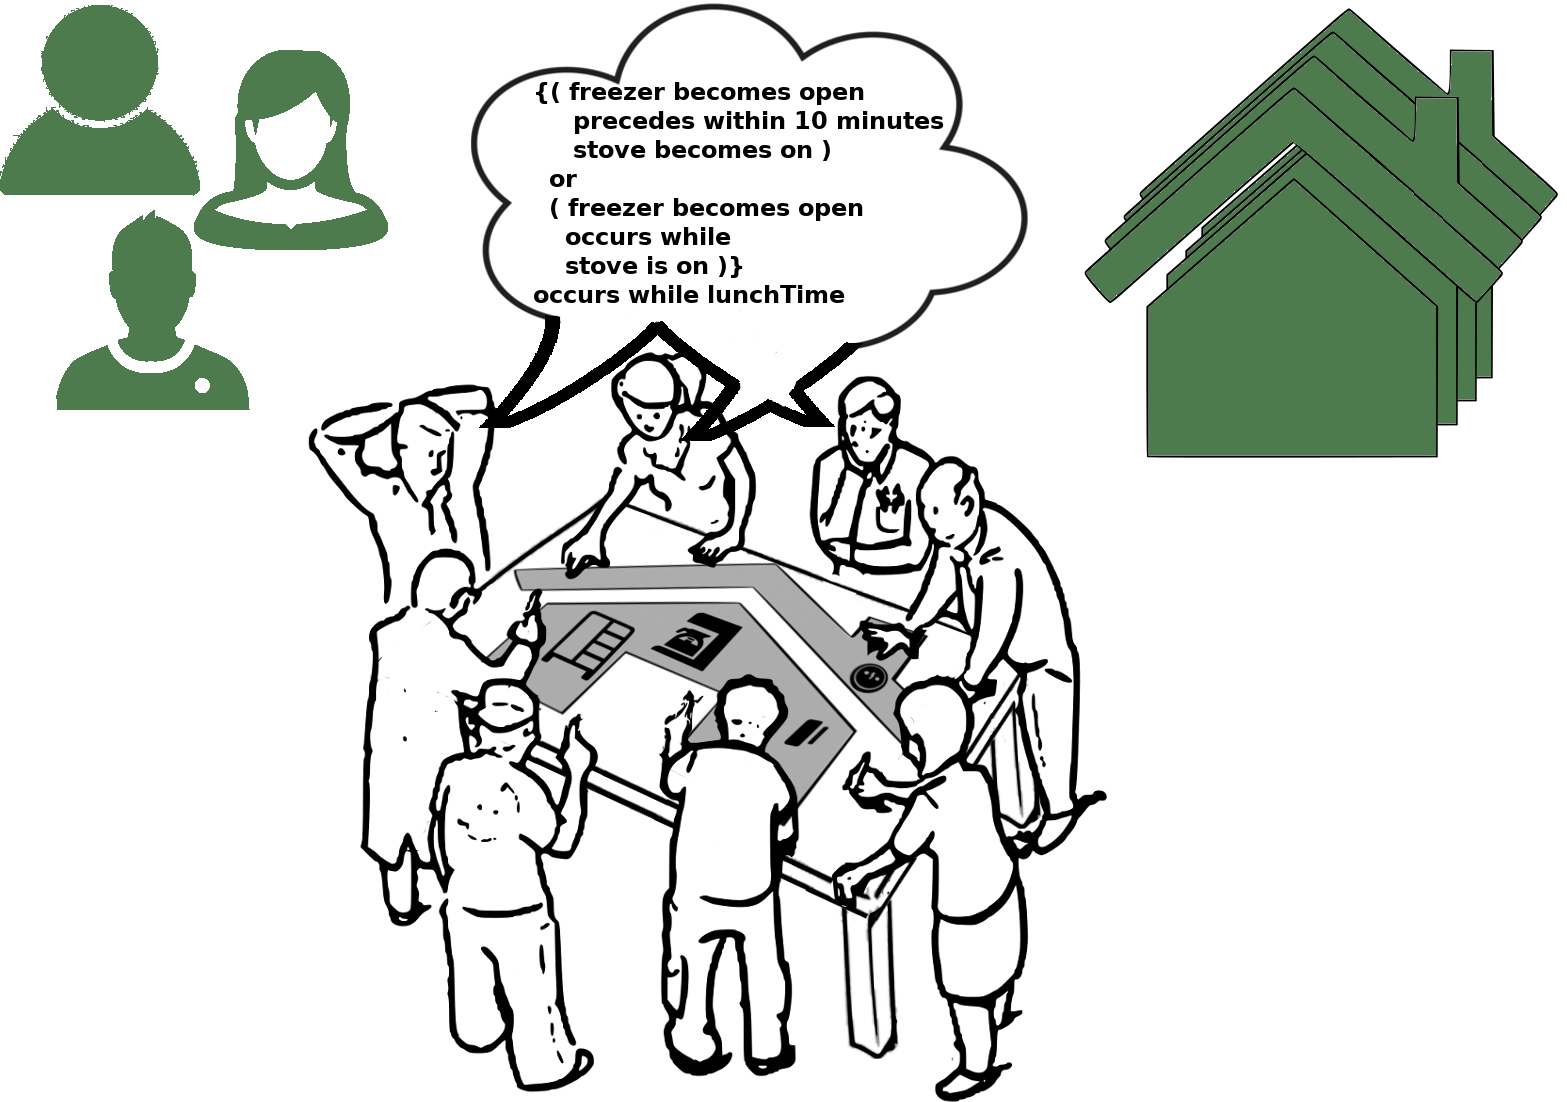
\includegraphics[scale=0.1]{axe_variation_final.png}
\end{minipage}
\vfill
Compilation masquant la complexité du traitement événementiel~:
\begin{itemize}
\item Services plus facile à exprimer et comprendre.
\end{itemize}

% Définition de services unifiée.
% \vfill
% Expressivité couvre les objectifs de services.
% \vfill
% Services plus facile à exprimer et comprendre.
% \vfill
% Modèle d'infrastructure exprimé avec des services.

% Unified approach to define services.\\
% Expessivity allow to cover objective of services.\\
% Model of infrastructure can be expressed as services.\\
% Services are easier to express than using Java.\\

\end{frame}

\begin{frame}{Perspectives}
\begin{minipage}{.5\linewidth}
Définition de services par les intervenants~:\\
\begin{itemize}
\item Étude ergonomique en cours \\(compréhension).
\item Langage graphique \\(programmation).
\end{itemize}
\end{minipage}
\hfill
\begin{minipage}{.45\linewidth}
\vspace*{3.11mm}
    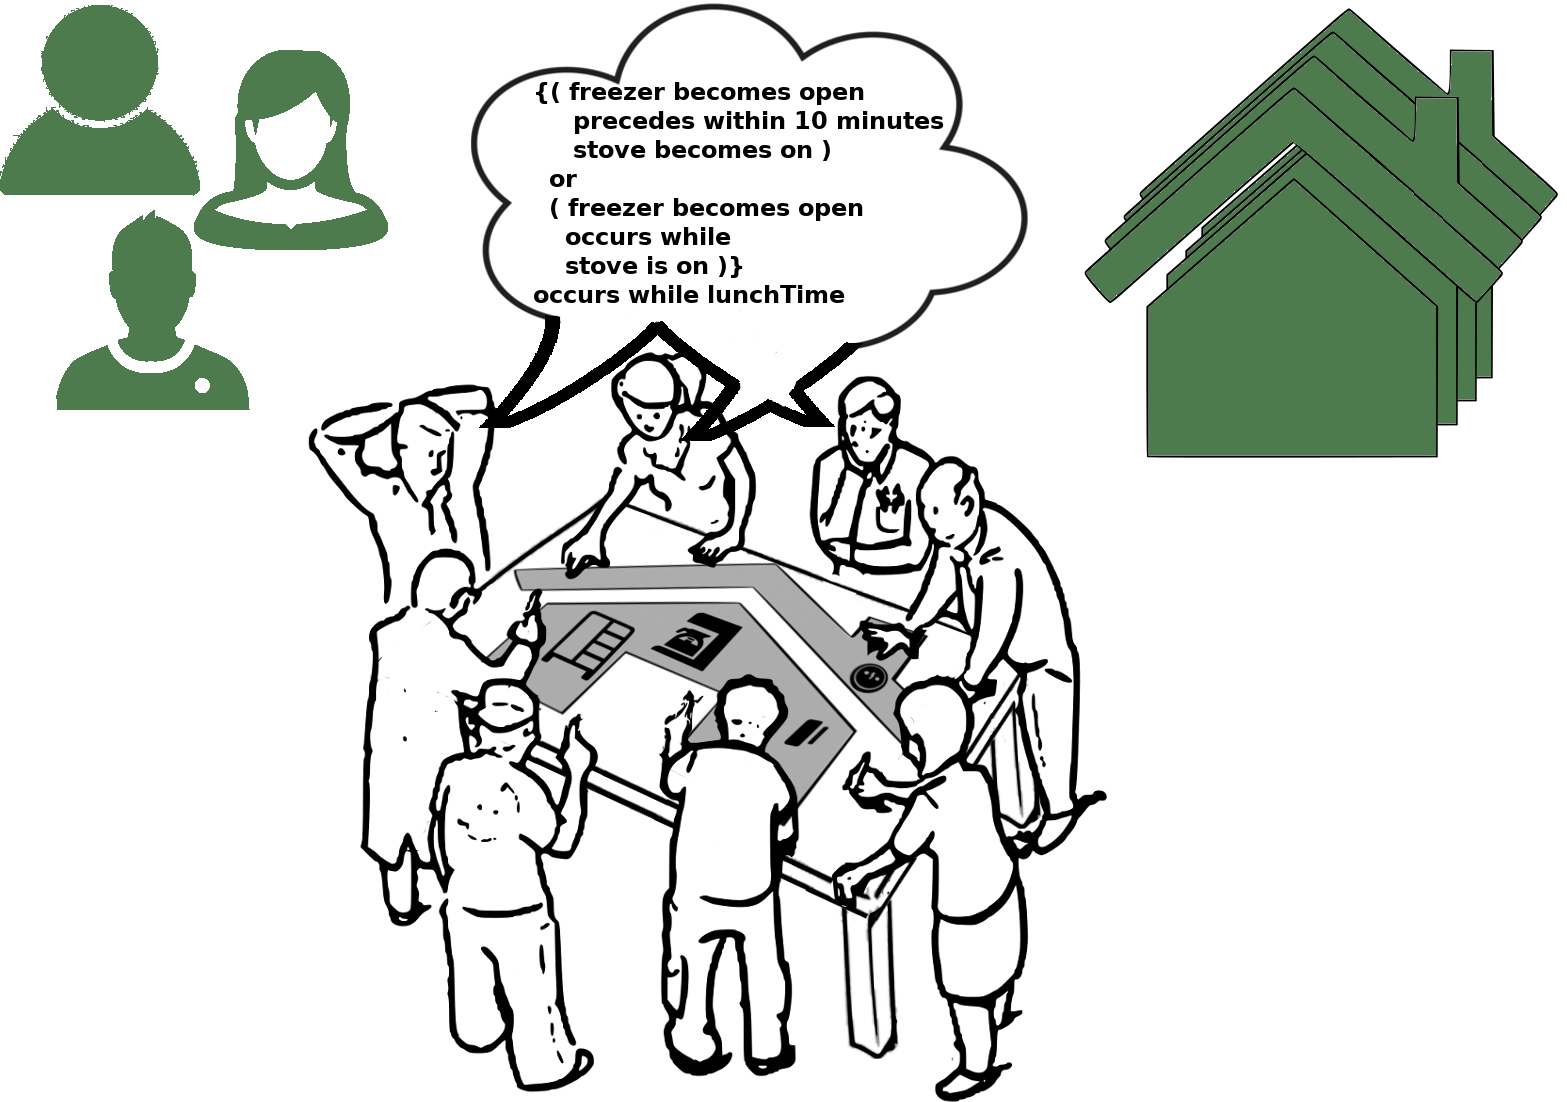
\includegraphics[scale=0.1]{axe_variation_final.png}
\end{minipage}
\vfill
Cibles de compilation~:\\
\begin{itemize}
\item Stream processing (Apache Spark, Flink).
%\item Couche graphique.
\end{itemize}
Évaluer le gain de l'éffort de développement.
% End-user service definition.\\
% Extend compilation targets.\\
\end{frame}